\section{Outliers}

To detecting outliers I started by creating a box plot for each feature.
\begin{figure}[H]
  \centering
  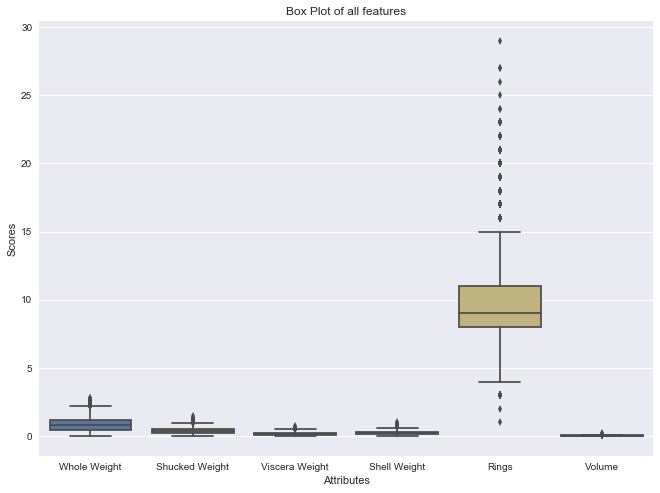
\includegraphics[scale=0.5,width=100mm]{./images/abalone-outlier-1.png}
  \caption{Box plot showing outliers for all features}
  \label{fig:abalone-outlier-1}
\end{figure}
Figure \ref{fig:abalone-outlier-1} shows a box plot for all features. Rings seems to be the most dominant feature in this plot, making it slightly hard to read. Lets take a look at a boxplot just for the rings feature.
\begin{figure}[H]
  \centering
  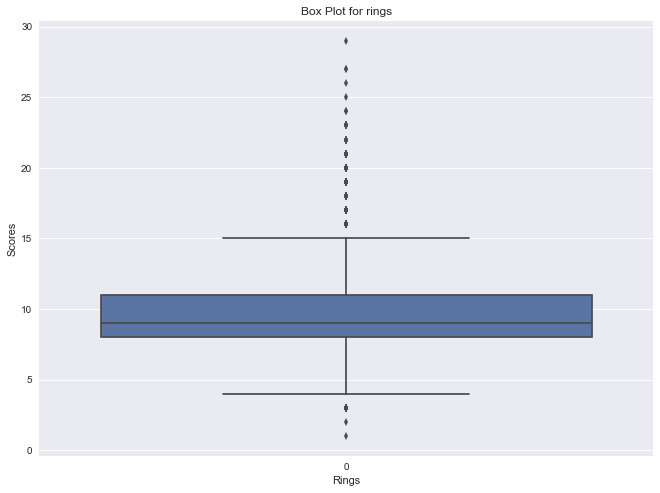
\includegraphics[scale=0.5,width=100mm]{./images/abalone-outlier-rings.png}
  \caption{Box plot showing outliers for rings feature}
  \label{fig:abalone-outlier-rings}
\end{figure}
Its hard to see from the plot in figure \ref{fig:abalone-outlier-rings}, but it turns out there are 278. I chose to drop all of these rows from the data-frame. For choosing the outliers I had to get the upper and lower whiskers. using the algorithm below
\begin{equation}
    1.5 \times IQR
\end{equation}
Where IQR is the inter-quartile range. I repeated this step for each feature with outliers. A summary of the total dropped per feature is listed below

\begin{itemize}
  \item \textbf{Whole Weight} 31
  \item \textbf{Shucked Weight} 20
  \item \textbf{Viscera Weight} 16
  \item \textbf{Shell Weight} 15
  \item \textbf{Volume} 5
\end{itemize}

This left me with a total of 3805 rows out of the original 4177. To confirm that all outliers have been removed I re-ran the box-plot as can be seen in figure \ref{fig:abalone-outlier-done}
\begin{figure}[H]
  \centering
  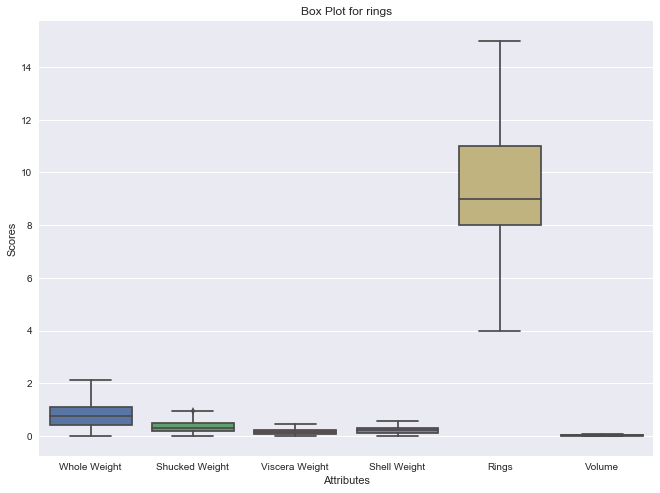
\includegraphics[scale=0.5,width=100mm]{./images/abalone-outlier-done.png}
  \caption{Box plot showing all outliers removed}
  \label{fig:abalone-outlier-done}
\end{figure}
